\begin{figure}[htbp]\centering
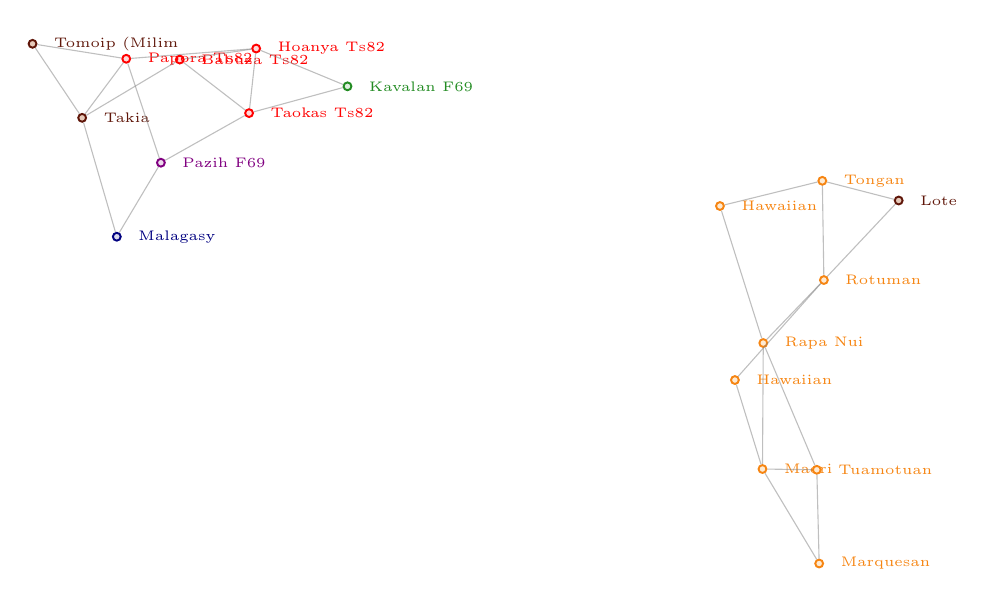
\begin{tikzpicture}[font=\scriptsize]
\node[circle,draw=BurntOrange,fill=BurntOrange!15,line width=0.7pt,inner sep=1pt] (L0) at (3.23,1.24) {};
\node[font=\tiny,BurntOrange,anchor=west] at (3.38,1.24) {Hawaiian};
\node[circle,draw=BurntOrange,fill=BurntOrange!15,line width=0.7pt,inner sep=1pt] (L1) at (3.77,-2.10) {};
\node[font=\tiny,BurntOrange,anchor=west] at (3.92,-2.10) {Maori};
\node[circle,draw=BurntOrange,fill=BurntOrange!15,line width=0.7pt,inner sep=1pt] (L2) at (4.53,1.56) {};
\node[font=\tiny,BurntOrange,anchor=west] at (4.68,1.56) {Tongan};
\node[circle,draw=NavyBlue,fill=NavyBlue!15,line width=0.7pt,inner sep=1pt] (L3) at (-4.43,0.85) {};
\node[font=\tiny,NavyBlue,anchor=west] at (-4.28,0.85) {Malagasy};
\node[circle,draw=BurntOrange,fill=BurntOrange!15,line width=0.7pt,inner sep=1pt] (L4) at (3.42,-0.97) {};
\node[font=\tiny,BurntOrange,anchor=west] at (3.57,-0.97) {Hawaiian};
\node[circle,draw=BurntOrange,fill=BurntOrange!15,line width=0.7pt,inner sep=1pt] (L5) at (4.46,-2.11) {};
\node[font=\tiny,BurntOrange,anchor=west] at (4.61,-2.11) {Tuamotuan};
\node[circle,draw=BurntOrange,fill=BurntOrange!15,line width=0.7pt,inner sep=1pt] (L6) at (4.55,0.30) {};
\node[font=\tiny,BurntOrange,anchor=west] at (4.70,0.30) {Rotuman};
\node[circle,draw=Sepia,fill=Sepia!15,line width=0.7pt,inner sep=1pt] (L7) at (-4.87,2.36) {};
\node[font=\tiny,Sepia,anchor=west] at (-4.72,2.36) {Takia};
\node[circle,draw=BurntOrange,fill=BurntOrange!15,line width=0.7pt,inner sep=1pt] (L8) at (3.78,-0.50) {};
\node[font=\tiny,BurntOrange,anchor=west] at (3.93,-0.50) {Rapa Nui};
\node[circle,draw=BurntOrange,fill=BurntOrange!15,line width=0.7pt,inner sep=1pt] (L9) at (4.49,-3.30) {};
\node[font=\tiny,BurntOrange,anchor=west] at (4.64,-3.30) {Marquesan};
\node[circle,draw=Red,fill=Red!15,line width=0.7pt,inner sep=1pt] (L10) at (-2.75,2.42) {};
\node[font=\tiny,Red,anchor=west] at (-2.60,2.42) {Taokas Ts82};
\node[circle,draw=Sepia,fill=Sepia!15,line width=0.7pt,inner sep=1pt] (L11) at (-5.50,3.30) {};
\node[font=\tiny,Sepia,anchor=west] at (-5.35,3.30) {Tomoip (Milim };
\node[circle,draw=Red,fill=Red!15,line width=0.7pt,inner sep=1pt] (L12) at (-2.66,3.24) {};
\node[font=\tiny,Red,anchor=west] at (-2.51,3.24) {Hoanya Ts82};
\node[circle,draw=Sepia,fill=Sepia!15,line width=0.7pt,inner sep=1pt] (L13) at (5.50,1.31) {};
\node[font=\tiny,Sepia,anchor=west] at (5.65,1.31) {Lote};
\node[circle,draw=ForestGreen,fill=ForestGreen!15,line width=0.7pt,inner sep=1pt] (L14) at (-1.50,2.76) {};
\node[font=\tiny,ForestGreen,anchor=west] at (-1.35,2.76) {Kavalan F69};
\node[circle,draw=Red,fill=Red!15,line width=0.7pt,inner sep=1pt] (L15) at (-3.63,3.10) {};
\node[font=\tiny,Red,anchor=west] at (-3.48,3.10) {Babuza Ts82};
\node[circle,draw=Purple,fill=Purple!15,line width=0.7pt,inner sep=1pt] (L16) at (-3.87,1.79) {};
\node[font=\tiny,Purple,anchor=west] at (-3.72,1.79) {Pazih F69};
\node[circle,draw=Red,fill=Red!15,line width=0.7pt,inner sep=1pt] (L17) at (-4.31,3.11) {};
\node[font=\tiny,Red,anchor=west] at (-4.16,3.11) {Papora Ts82};
\draw[gray,opacity=0.5,line width=0.4pt] (L0) -- (L2);
\draw[gray,opacity=0.5,line width=0.4pt] (L0) -- (L8);
\draw[gray,opacity=0.5,line width=0.4pt] (L1) -- (L5);
\draw[gray,opacity=0.5,line width=0.4pt] (L1) -- (L8);
\draw[gray,opacity=0.5,line width=0.4pt] (L1) -- (L4);
\draw[gray,opacity=0.5,line width=0.4pt] (L1) -- (L9);
\draw[gray,opacity=0.5,line width=0.4pt] (L2) -- (L6);
\draw[gray,opacity=0.5,line width=0.4pt] (L2) -- (L13);
\draw[gray,opacity=0.5,line width=0.4pt] (L3) -- (L16);
\draw[gray,opacity=0.5,line width=0.4pt] (L3) -- (L7);
\draw[gray,opacity=0.5,line width=0.4pt] (L4) -- (L6);
\draw[gray,opacity=0.5,line width=0.4pt] (L5) -- (L8);
\draw[gray,opacity=0.5,line width=0.4pt] (L5) -- (L9);
\draw[gray,opacity=0.5,line width=0.4pt] (L6) -- (L8);
\draw[gray,opacity=0.5,line width=0.4pt] (L6) -- (L13);
\draw[gray,opacity=0.5,line width=0.4pt] (L7) -- (L17);
\draw[gray,opacity=0.5,line width=0.4pt] (L7) -- (L15);
\draw[gray,opacity=0.5,line width=0.4pt] (L7) -- (L11);
\draw[gray,opacity=0.5,line width=0.4pt] (L10) -- (L12);
\draw[gray,opacity=0.5,line width=0.4pt] (L10) -- (L16);
\draw[gray,opacity=0.5,line width=0.4pt] (L10) -- (L14);
\draw[gray,opacity=0.5,line width=0.4pt] (L10) -- (L15);
\draw[gray,opacity=0.5,line width=0.4pt] (L11) -- (L17);
\draw[gray,opacity=0.5,line width=0.4pt] (L12) -- (L17);
\draw[gray,opacity=0.5,line width=0.4pt] (L12) -- (L14);
\draw[gray,opacity=0.5,line width=0.4pt] (L12) -- (L15);
\draw[gray,opacity=0.5,line width=0.4pt] (L16) -- (L17);
\end{tikzpicture}
\caption{\textbf{Language graph $G_L$ of Austronesian.} Each node is a language, coloured by its Glottolog branch; two languages are joined when one is among the other's two nearest neighbours in \emph{operator-distribution} distance (Jensen--Shannon). Colour was \emph{not} used to build the graph --- only the operator frequencies were. Whether same-colour nodes cluster is a visual test of how much genealogy the distributions alone carry (cf.\ Chapters 14, 18). Branches: \textcolor{NavyBlue}{Basap-Greater Barito}, \textcolor{BurntOrange}{Central Pacific linkage}, \textcolor{ForestGreen}{East Formosan}, \textcolor{Purple}{Northwest Formosan}, \textcolor{Sepia}{Western Oceanic linkage}, \textcolor{Red}{Western Plains Austronesian}.}
\end{figure}
